\label{section:vertex-area-chapter}
This section shows alternative methods to extend the idea of flat shading from triangles to vertices and edges. The idea of flat shading is to draw all the pixels of a triangle with the same colour. The extension of this approach is to split the surface of the triangle mesh likewise into regions around vertices and edges and draw all pixels in these regions with the same colour (Fig. \ref{fig:vertex-area}), thus visualizing data given at the vertices or edges of the mesh in a piecewise constant, not necessarily continuous way, resembling the classical triangle flat shading. The aforementioned regions can easily be defined using barycentric coordinates and a simple GPU fragment program (Fig. \ref{fig:max-diagram}) can be used to find out for each pixel to which region is belongs and which colour it should be painted with.

%%%%%%%%%%%%%


\begin{figure}[h]
    \centering
    \minipage[b]{.5\linewidth}
    \centering
    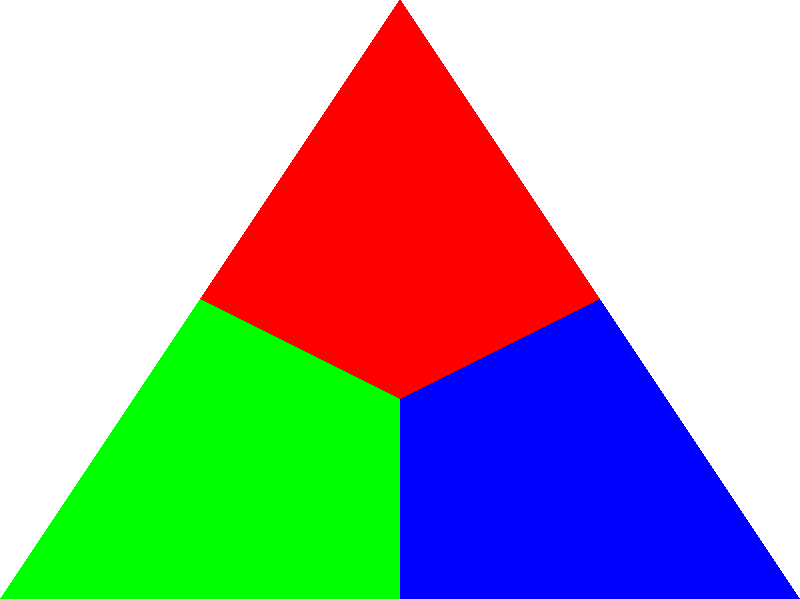
\includegraphics[scale=0.15]{images/max.png}
    \caption{Max diagram}\label{fig:max-diagram}
    \endminipage\hfill
    \minipage[b]{.5\linewidth}
    \centering
    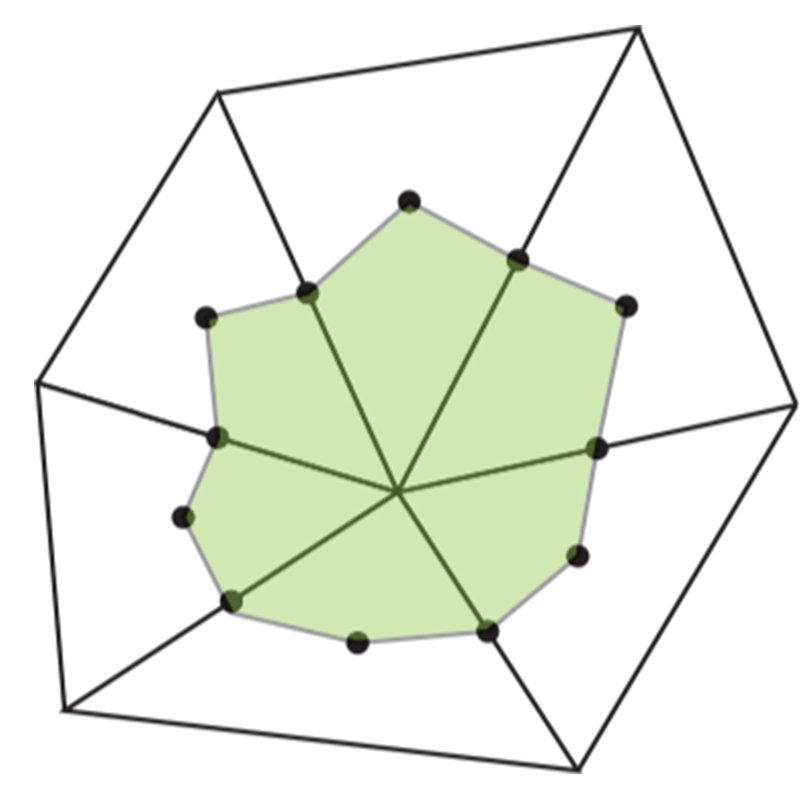
\includegraphics[scale=0.15]{images/vertex-area.png}
    \caption{Region around a vertex}\label{fig:vertex-area}
    \endminipage
\end{figure}

%%%%%%%%%%%%%

\subsection{Max diagram - Vertex based area} \label{section:max-diagram}
Passing barycentric coordinates to the \textit{fragment shader} will clearly demonstrate that we can get results different from the classic color interpolation.
\cite{WEBSITE:redbloggames}
%----------
There are different approaches to color interpolation focusing on the distance from vertices. For each point in a triangle, we can easily determine its closest vertex, which we use as a cue for coloring.
A different approach from interpolating, can be found coloring vertex areas based on the minimum barycentric coordinate.
The color is given by the region farthest from a vertex (Fig. \ref{fig:max-diagram}, Pseudocode \ref{appendix:max-diagram}).

%%%%%%%%%%%%%

\subsection{Flat shading extension} \label{section:extend-flat-shading-lighting}
An extension of \textit{flat shading} would be to have each vertex area to be in one constant color. This color can be taken from shading interpolation using the normal at the vertex and the vertex position.
The color will then be computed as in \textit{Gouraud shading}.
The idea is to compute the color per vertex but instead of linearly interpolated it in each triangle (as \textit{Gouraud shading} does) we color regions around a vertex with that constant color.
To implement it, the barycentric coordinates, the vertex color, the normal at the vertex and the lighting calculations must be passed to the \textit{fragment shader}.
We want to avoid an automatic interpolation of colors, in order to return the resulting color using the \textit{max diagram} we have used a \textit{Geometry shader} that have access to all three vertex colors in \textit{fragment shader}. (Pseudocodes: \ref{appendix:vs-flat-shading-lighting}, \ref{appendix:gs-flat-shading-lighting}, \ref{appendix:fs-flat-shading-lighting})

\subsubsection{Comparison}
Gouraud shading vs extension flat shading.
TODO

%%%
\subsection{Discrete Gaussian Curvature}
\label{section:vertex-area-gaussian-curvature}
Another interesting alternative data visualization technique is to compute the \textit{Gaussian curvature} per vertex. That can be done summing up, for each vertex, angles at this vertex with adjacent triangles and then subtracting this value to $2\pi$.
After having obtain this value, called \textit{angle defect} (Fig. \ref{fig:gc-angle}), we map linearly this value to a color range.
The resulting color will be the vertex flat shading visualisation of \textit{Gaussian curvature}.
$$K(V) = 2\pi - \sum_j \theta_j$$
%%
\begin{figure}[!h]
    \centering
    \begin{tikzpicture}
        \coordinate (J) at (3.1,2.9);
        \coordinate (circle) at (3.1,2.9);
        \node[anchor=south west,inner sep=0] at (0,0) {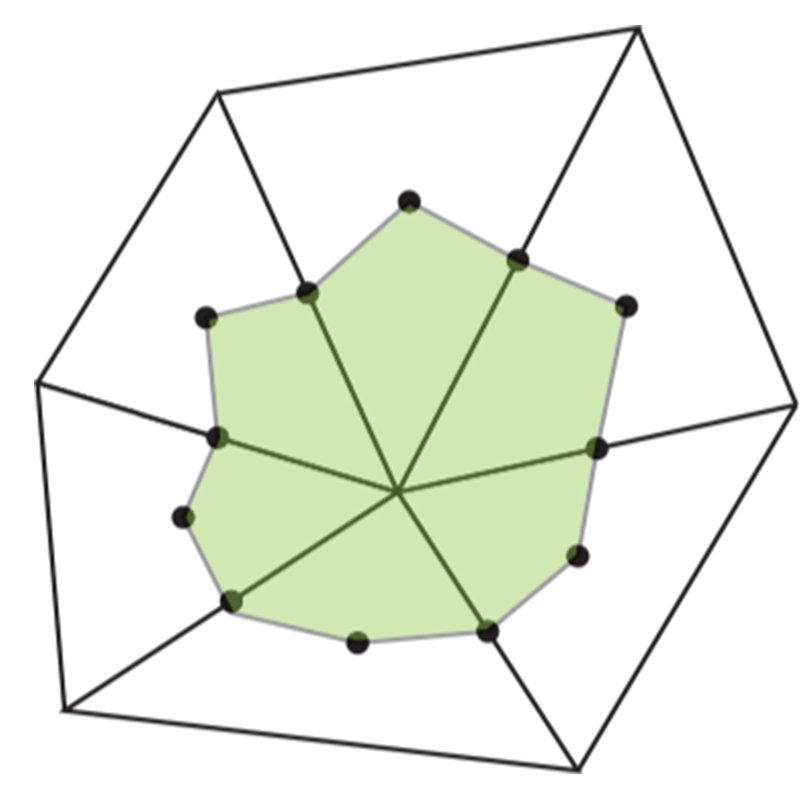
\includegraphics[scale=0.2]{images/vertex-area.png}};
        \draw (J) node [below left] {$j$};
        \filldraw (2.8, 2.2) circle (2pt);
        \begin{scope}[line width=0.4mm, line cap=round]
            \draw (3.2,1.7) arc (295:360:0.7cm) node[near start,right] {$\theta_j$};
        \end{scope}
    \end{tikzpicture}
    \caption{Angle defect}\label{fig:gc-angle}
\end{figure}
%%
\textit{Gaussian curvature} returns a constant color around each vertex (Fig. \ref{fig:gc-icosahedron}, Pseudocode \ref{appendix:vs-gaussiancurvature}).
\begin{figure}[h]
    \centering
    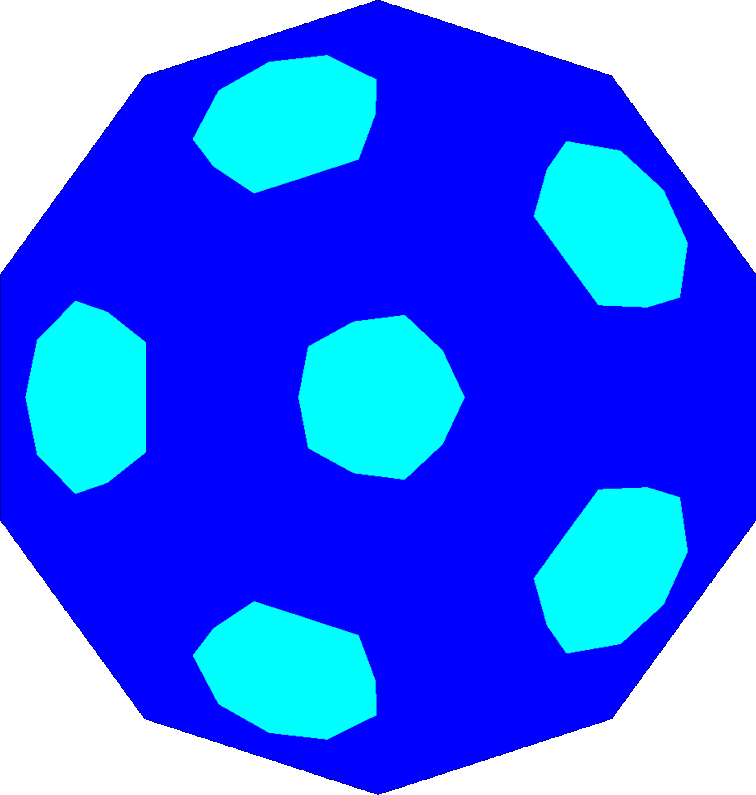
\includegraphics[scale=0.2]{images/gaussian-ball.png}
    \caption{Gaussian curvature on icosahedron}\label{fig:gc-icosahedron}
\end{figure}
TODO: update image 3.4
%%%%%%%%

\subsection{Interpolated Gaussian Curvature}
aka Gouraud Shading Gaussian Curvature
TODO

\subsubsection{Comparison}
We want now to compare the \textit{Gaussian curvature} (Fig. \ref{fig:gaussian-interpolated-horse}) with the \textit{interpolated Gaussian curvature}. In Fig. \ref{fig:gaussian-horse} each vertex area is colored applying the method \textit{max diagram} described in the above subsection \ref{section:max-diagram}. Instead, in Fig. \ref{fig:gaussian-interpolated-horse} the color is obtained with a linear interpolation.
\begin{figure}[!htb]
\centering
  \minipage{0.4\textwidth}
    % \includegraphics[width=\linewidth]{images/}
    \caption{Interpolated Gaussian curvature} \label{fig:gaussian-interpolated-horse}
  \endminipage\hfill
  \centering
  \minipage{0.4\textwidth}%
    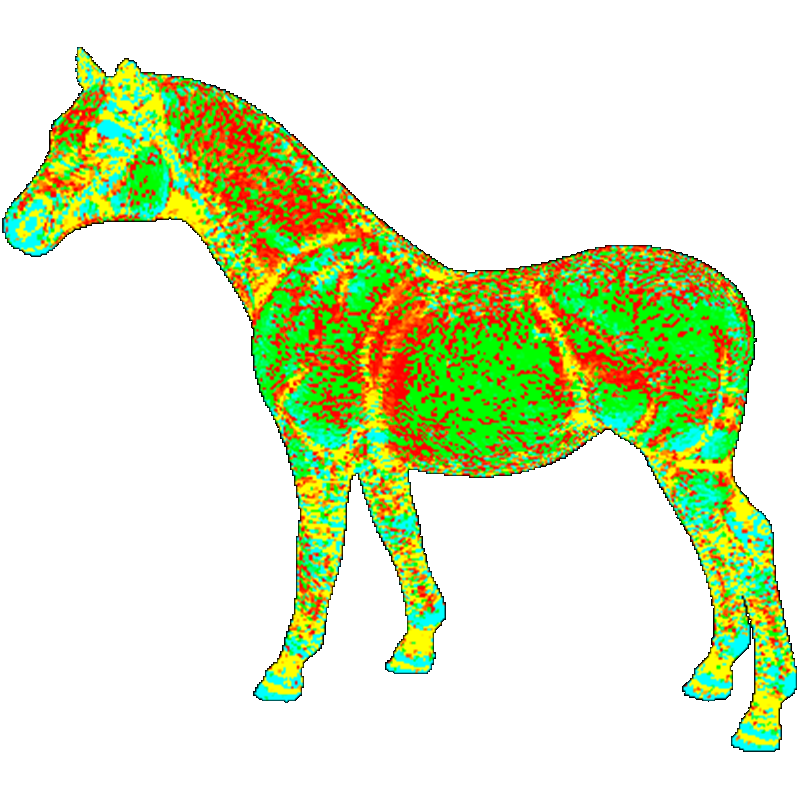
\includegraphics[width=\linewidth]{images/gaussian-horse.png}
    \caption{Gaussian curvature}\label{fig:gaussian-horse}
  \endminipage
  \end{figure}

Visualization of the principal curvatures of the model as colors from blue (highest values of curvature) to red (lower values of curvature), in both Fig. \ref{fig:gaussian-horse} and Fig. \ref{fig:gaussian-interpolated-horse}, better highlighs the geometry of the horse.
These changes of curvature, positive (blue), flat (green) and negative regions (red), better emphasises the 3-dimensionality of the model.
TODO
% \textit{Gaussian curvature} better shows the muscle constrasts given a more realistic character to the horse than the model obtained using the \textit{interpolated Gaussian curvature}.
